\documentclass[10pt,a4paper]{article}
\usepackage[utf8]{inputenc}
\usepackage{amsmath}
\usepackage{tikz} 
\usepackage{amsfonts}
\usepackage{amssymb}
\author{David Cerna}
\title{Wordle is NP-Complete}
\newtheorem{definition}{Definition}
\begin{document}
\maketitle
\section{Dominating Set Cover}
Let $k\geq 1$,  and $G = (V, E)$ an undirected graph. Does there exists $D\subseteq V$ of size $\leq k$ such that for every $v\not \in D$ there exists a $w\in D$ such that $(v,w)\in E$.

\section{Wordle}
Let $\mathcal{A}= \{\alpha_{i}\}^{l}_{i=1}$ be an alphabet, $\mathcal{A}^{m} =\{ \alpha_{i_1}\cdots \alpha_{i_m}\vert 1\leq j\leq m\ \& \ 1\leq i_j\leq l\}$,  $S\subseteq A^m$, $t\in S$, and  $f_t:S\rightarrow \{0,1,2\}^m$ is a scoring function, defined as $f_t(w) = \left\langle f_t^1(w),\cdots, f_t^{m}(w)\right\rangle$ where
$$f_t^i(w) =\left\lbrace \begin{array}{cc}
0 &  w_i = t_i \\
1 & w_i \not = t_i\ \&\ \exists j(w_i = t_j \ \& \ \forall k< i(w_k =w_i \rightarrow \exists r< j (w_k=t_r)))\\
2 & otherwise
\end{array}\right.$$
Does there exists a subset $S'$ of $S\setminus \{t\}$ such that $\vert S'\vert \leq n< \vert S\vert-1 $ and $t$ is the only word not excluded by the set of constraints $\{f_t(w)\vert w\in S'\}$?

\begin{definition}
For $w,w'\in S$, we say that $f_t(w)$ excludes a word $w'$ if one of the following holds: 

\begin{itemize}
\item $f_t^i(w) = 0$ and $w_i\not= w'_i $. 
\item $f_t^i(w) = 1$ and $w_i \not \in w'$.
\item $f_t^i(w) = 2$, $\forall j( w_i = w_j\rightarrow f_t^j(w) = 2)$ and $w_i\in w'$.
\item $f_t^i(w) = 2$,  $\exists j( w_i = w_j \ \&\ f_t^j(w) < 2 \ \& \ \vert\{j\vert w_i=w_j\}\vert\leq \vert\{j\vert w_i=w'_j\}\vert)$.
\end{itemize}
\end{definition}

\section{Reduction from dominating set to Wordle}
First we need to construct a graph $K = (V,E')$ such that $E' =B\cup R$ where $B=E$ and $R =\{ (v,w)\vert v,w\in V \ and \ (v,w)\not \in E\}$. Let $\mathit{NR}(v) =\{ (v,w)\vert w\in V,\ and \ (v,w)\in R\}$ and
$\mathit{NB}(v) =\{ (v,w)\vert w\in V,\ and \ (v,w)\in B\}$.


Note that $K$ is complete. Our alphabet $\mathcal{A}$ contains 
$\vert V\vert^2\vert B\vert$ letters which we denote as follows
$$\{\alpha_{i}\}^{\vert B\vert}_{i=1}\cup \{\beta_{i}\}^{(\vert V\vert^2-1)\vert B\vert}_{i=1}$$

In total we construct $\vert V\vert+1$ words denoted by $\{ t\}\cup \{w^{i}\}^{\vert V\vert}_{i=1}$. Let $ B  = \{b_{i}\}^{\vert B\vert}
_{i=1}$, $ R  = \{r_{i}\}^{\vert R\vert}
_{i=1}$, and  $ V  = \{v_{i}\}^{\vert V\vert}_{i=1}$, then 
\begin{itemize}

\item for $1\leq i \leq \vert B\vert$, if $b_i = (v_j,v_k)$, then $w^j_i=w^k_i=\alpha_i$.

\item for $1\leq i \leq \vert V\vert$ and $\vert B\vert +1+\sum_{k=1}^{i-1} \mathit{NR}(V_{k})\leq l\leq j \leq \vert B\vert +1+\sum_{k=1}^{i} \mathit{NR}(V_{k}),$ $w^i_j \in \{\alpha_{i}\}^{\vert B\vert}_{i=1}$ such that $w^i_j \not = w^i_l$ iff $j\not = l$, and for all $1\leq q \leq \vert B\vert$, $w^i_j\not = w^i_q$. 
\item $1\leq i \leq \vert B\vert$, $t_{i+\vert B\vert +1+\sum_{k=1}^{\vert V\vert} \mathit{NR}(V_{k})} = \alpha_i$
\item All positions not mentioned contain a unique symbol from $\{\beta_{i}\}^{(\vert V\vert^2-1)\vert B\vert}_{i=1}$.

Notice, each of these words is $\vert V\vert \vert B\vert$ long. 
\section{example}

The graph below has a minimal dominating sets of $\{ v_3,v_5\}$ and $\{ v_2,v_5\}$.
\begin{center}
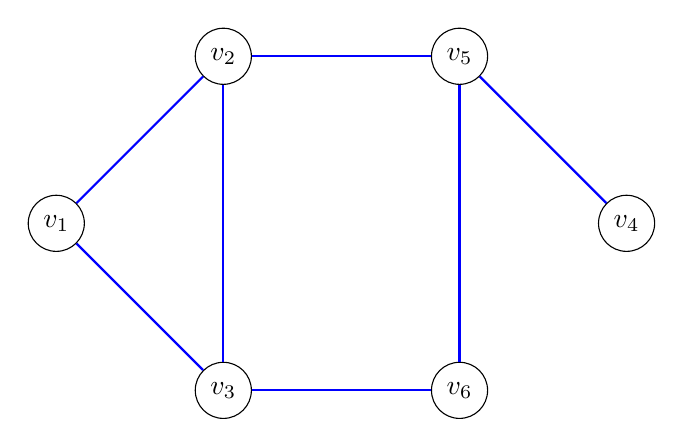
\begin{tikzpicture}[main/.style = {draw, circle}, node distance={30mm}] 
\node[main] (1) {$v_1$}; 
\node[main] (2) [above right of=1] {$v_2$};
\node[main] (3) [below right of=1] {$v_3$}; 
\node[main] (5) [ right of=2] {$v_5$}; 
\node[main] (6) [ right of=3] {$v_6$};
\node[main] (4) [ above right of=6] {$v_4$};
\draw[blue,thick] (1) -- (2);
\draw[blue,thick] (1) -- (3);
\draw[blue,thick] (2) -- (3);
\draw[blue,thick] (2) -- (5);
\draw[blue,thick] (3) -- (6);
\draw[blue,thick] (4) -- (5);
\draw[blue,thick] (5) -- (6);
\end{tikzpicture} 
\end{center}

We transform the graph preserving the edges using colors. 
\begin{center}
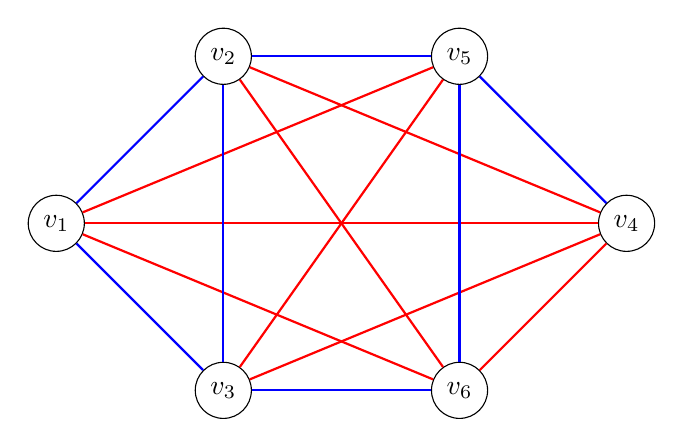
\begin{tikzpicture}[main/.style = {draw, circle}, node distance={30mm}] 
\node[main] (1) {$v_1$}; 
\node[main] (2) [above right of=1] {$v_2$};
\node[main] (3) [below right of=1] {$v_3$}; 
\node[main] (5) [ right of=2] {$v_5$}; 
\node[main] (6) [ right of=3] {$v_6$};
\node[main] (4) [ above right of=6] {$v_4$};
\draw[blue,thick] (1) -- (2);
\draw[blue,thick] (1) -- (3);
\draw[red,thick] (1) -- (4);
\draw[red,thick]  (1) -- (5);
\draw[red,thick]  (1) -- (6);
\draw[blue,thick] (2) -- (3);
\draw[red,thick]  (2) -- (4);
\draw[blue,thick] (2) -- (5);
\draw[red,thick]  (2) -- (6);
\draw[red,thick]  (3) -- (4);
\draw[red,thick]  (3) -- (5);
\draw[blue,thick] (3) -- (6);
\draw[blue,thick] (4) -- (5);
\draw[red,thick]  (4) -- (6);
\draw[blue,thick] (5) -- (6);
\end{tikzpicture} 
\end{center}
\end{itemize}

From the transformed graph we need to construct words for each vertex. The idea is that words connected by a blue edge exclude each other and words connected by a red edge don't. 

$$\begin{array}{c|ccccccccccccccccccccccc}
&1&2&3&4&5&6&7&8&9&10&11&12&13&14&15&16 \\\hline

v_1&\bullet&\bullet&\alpha_3&\bullet&\bullet&\bullet&\alpha_7&\bullet&\bullet&\bullet&\bullet&\bullet&\bullet&\bullet&\bullet&\bullet
\\
v_2 &\alpha_1 & \alpha_2&\alpha_3&\bullet&\bullet&\bullet&\bullet&\alpha_4&\alpha_5&\alpha_6&\alpha_7&\bullet&\bullet&\bullet&\bullet&\bullet
\\
v_3&\bullet&\alpha_2&\bullet&\bullet&\bullet&\alpha_6&\alpha_7&\bullet&\bullet&\bullet&\bullet&\bullet&\bullet&\bullet&\bullet&\bullet
\\
v_4&\bullet&\bullet&\bullet&\alpha_4&\bullet&\bullet&\bullet&\bullet&\bullet&\bullet&\bullet&\bullet&\bullet&\bullet&\bullet&\alpha_1
\\
v_5&\alpha_1&\bullet&\bullet&\alpha_4&\alpha_5&\bullet&\bullet&\bullet&\bullet&\bullet&\bullet&\alpha_2&\alpha_3&\alpha_6&\alpha_7&\bullet&
\\
v_6&\bullet&\bullet&\bullet&\bullet&\alpha_5&\alpha_6&\bullet&\bullet&\bullet&\bullet&\bullet&\bullet&\bullet&\bullet&\bullet&\bullet&
\\
t&\bullet&\bullet&\bullet&\bullet&\bullet&\bullet&\bullet&\bullet&\bullet&\bullet&\bullet&\bullet&\bullet&\bullet&\bullet&\bullet

\end{array}$$

$$\begin{array}{c|cccccccccccccccccccccccccccccccccccccccccc}
&17&18&19&20&21&22&23&24&25&26&27&28&29&30&31&32\ \\\hline

v_1&\bullet&\bullet&\bullet&\bullet&\bullet&\bullet&\bullet&\bullet&\bullet&\bullet&\bullet&\bullet&\bullet&\bullet&\alpha_1&\alpha_2&
\\
v_2 &\bullet&\bullet&\bullet&\bullet&\bullet&\bullet&\bullet&\bullet&\bullet&\bullet&\bullet&\bullet&\bullet&\bullet&\bullet&\bullet
\\
v_3&\bullet&\bullet&\bullet&\bullet&\bullet&\bullet&\bullet&\bullet&\bullet&\bullet&\alpha_1&\alpha_3&\alpha_4&\alpha_5&\bullet&\bullet
\\
v_4&\alpha_2&\alpha_3&\alpha_5&\alpha_6&\alpha_7&\bullet&\bullet&\bullet&\bullet&\bullet&\bullet&\bullet&\bullet&\bullet&\bullet&\bullet
\\
v_5&\bullet&\bullet&\bullet&\bullet&\bullet&\bullet&\bullet&\bullet&\bullet&\bullet&\bullet&\bullet&\bullet&\bullet&\bullet&\bullet
\\
v_6&\bullet&\bullet&\bullet&\bullet&\bullet&\alpha_1&\alpha_2&\alpha_3&\alpha_4&\alpha_7&\bullet&\bullet&\bullet&\bullet&\bullet&\bullet
\\
t&\bullet&\bullet&\bullet&\bullet&\bullet&\bullet&\bullet&\bullet&\bullet&\bullet&\bullet&\bullet&\bullet&\bullet&\bullet&\bullet

\end{array}$$


$$\begin{array}{c|cccccccccccccccccccccccccccccccccccccccccc}
&33&34&35&36&37&38&39&40&41&42\ \\\hline

v_1&\alpha_4&\alpha_5&\alpha_6&\bullet&\bullet&\bullet&\bullet&\bullet&\bullet&\bullet
\\
v_2 &\bullet&\bullet&\bullet&\bullet&\bullet&\bullet&\bullet&\bullet&\bullet&\bullet
\\
v_3&\bullet&\bullet&\bullet&\bullet&\bullet&\bullet&\bullet&\bullet&\bullet&\bullet
\\
v_4&\bullet&\bullet&\bullet&\bullet&\bullet&\bullet&\bullet&\bullet&\bullet&\bullet
\\
v_5&\bullet&\bullet&\bullet&\bullet&\bullet&\bullet&\bullet&\bullet&\bullet&\bullet
\\
v_6&\bullet&\bullet&\bullet&\bullet&\bullet&\bullet&\bullet&\bullet&\bullet&\bullet
\\
t&\bullet&\bullet&\bullet&\alpha_1&\alpha_2&\alpha_3&\alpha_4&\alpha_5&\alpha_6&\alpha_7

\end{array}$$

Bullets are chosen uniquely from $ \{\beta_{i}\}^{245}_{i=1}$. Notice that $\{w_2, w_5\}$, and  $\{w_2, w_5\}$ cover all words but the target $t$. All other sets of words do not cover the whole set or contain more words.  
\end{document}